\chapter{Modélisation}
\label{chapter-1}
\section{Hypothèses physiques}

\subsection{Hypoth{\`e}ses de d{\'e}part}

Pour simplifier la r{\'e}alisation du code, plusieurs simplifications
g{\'e}om{\'e}triques et physiques ont {\'e}t{\'e} prises en compte.

\subsubsection*{Sp{\'e}cificit{\'e}s du r{\'e}seau}

Notre couverture de base est assur{\'e}e par une antenne dip{\^o}le $\lambda /
2$, celle-ci sera consid{\'e}r{\'e}e sans perte. Elle {\'e}mettra avec une
fr{\'e}quence de 60 GHz (suivant la norme Wi-Fi IEEE 802.11 ay) et avec une
puissance de 20 dBm. Pour la r{\'e}ception, nous consid{\'e}rons un seuil
minimal de -90 dBm et un seuil maximal de -40 dBm. Les d{\'e}bits binaires
correspondants valent respectivement 50 Mb/s et 40 Gb/s.

\subsubsection*{G{\'e}om{\'e}trie du probl{\`e}me}

Nous ne prendrons en compte que deux dimensions de l'espace, c'est {\`a} dire
que nous consid{\'e}rons que les antennes sont plac{\'e}es {\`a} une m{\^e}me
hauteur sur l'axe $z$ et n'{\'e}mettent et ne recoivent que dans la dimension
transverse {\`a} celui-ci. Nous ne consid{\'e}rons donc
que les dimensions $(x, y)$ de nos murs.

\subsubsection*{Simulation de la couverture de base}

L'{\'e}tude de la couverture de base de la borne Wi-Fi se fait via la
m{\'e}thode des images (d{\'e}taill{\'e}e plus loin) qui nous permettra de
tracer le trajet des rayons entre l'antenne {\'e}mettrice et l'antenne
r{\'e}ceptrice. On consid{\'e}rera les rayons transmis {\`a} travers les
murs, et les ondes r{\'e}fl{\'e}chies avec un maximum de deux r{\'e}flexions.
On ne prendra pas en compte la diffraction des ondes.

\subsection{Hypoth{\`e}se de champ lointain}

Afin d'utiliser nos m{\'e}thodes de trac{\'e} de rayon, nous allons
d{\'e}terminer dans quel cadre th{\'e}orique on se place. Les dimensions de
notre probl{\`e}me nous imposent de travailler sous les hypoth{\`e}ses de
\textit{champ lointain}.

La fronti{\`e}re de champ lointain est d{\'e}finie avec
\[ r_f = \max \left\{ 1.6 \lambda, 5 D, \frac{2 D^2}{\lambda} \right\} \]
avec $D$ la dimension du circuit {\'e}metteur et $\lambda$ la longueur d'onde
d{\'e}duite de la fr{\'e}quence de travail $f$. Nos {\'e}metteurs sont des
{\'e}metteurs de type $\lambda / 2$, leur dimension vaut donc
approximativement $\lambda / 2$. Notre fr{\'e}quence de travail est celle du
Wi-Fi IEEE 802.11ay et donc $f = 60 \mathrm{GHz}$. On peut donc {\'e}valuer $\lambda$
via
\[ \lambda = \frac{c}{f} = 5 \cdot 10^{- 3} \mathrm{m} \]
On en d{\'e}duit que $r_f = 5 D = 1.25 \mathrm{cm}$ et que donc notre
approximation est donc tout {\`a} fait valable car notre espace est
d{\'e}coup{\'e} en carr{\'e}s de 0.5m de largeur.

\subsection{Propri{\'e}t{\'e}s des antennes $\lambda / 2$}

Les propri{\'e}t{\'e}s des antennes dip{\^o}les, dites $\lambda / 2$, ont
{\'e}t{\'e} {\'e}tudi{\'e}es au cours, dans le chapitre relatif aux antennes,
d'o{\`u} nous d{\'e}duirons nos {\'e}quations. Dans notre cas, l'antenne n'a pas de
pertes et une r{\'e}sistance $R_a = 73 \Omega$. Plac{\'e}e sur l'axe $z$, sa
hauteur {\'e}quivalente s'exprime comme
\[ \vec{h}_e (\theta, \phi) = - \frac{\lambda \cos \left( \frac{\pi}{2} \cos
   \theta \right)}{\pi \sin^2 \theta} \vec{1}_z \]
Cependant, comme {\'e}nonc{\'e} plus haut, nous n'allons consid{\'e}rer que
deux dimensions de l'espace, et donc nous prendrons $\theta = \frac{\pi}{2}$.
\[ \vec{h}_e \left( \frac{\pi}{2}, \phi \right) = - \frac{\lambda}{\pi}
   \vec{1}_z \]
Nous prendrons cette valeur en compte dans le calcul des puissances.

\section{Propagation des ondes}

Les formules de cette section sont issues du cours, principalement du chapitre
relatif aux calculs de coefficients de r{\'e}flexion, transmission et
diffraction.

\subsection{Propri{\'e}t{\'e}s des murs}

Les champs se propageront soit dans l'air (assimil{\'e} au vide) soit en
traversant et/ou en se r{\'e}fl{\'e}chissant sur des murs. Pour calculer les
effets relatifs {\`a} ces interactions entre les murs et les ondes, on
utilisera leurs propri{\'e}t{\'e}s {\'e}lectriques. Ces propri{\'e}t{\'e}s
sont donn{\'e}es par la constante de propagation dans un mat{\'e}riau
%\[ \gamma_m = \alpha_m + j \beta_m = \sqrt{j \omega \mu (\sigma + j \omega
%   \varepsilon)} \]
\[ \gamma_m = \alpha_m + j \beta_m = j\omega \sqrt{\mu_0 \tilde{\varepsilon}} \]
%avec $\sigma$ la conductivit{\'e} et $\varepsilon$ la permettivit{\'e} du
avec $\tilde{\varepsilon}$ la permittivité complexe
($\tilde{\varepsilon} = \varepsilon_r\varepsilon_0 - j\frac{\sigma}{\omega}$, où
$\varepsilon_r$ est la permittivité relative, et $\sigma$ la conductivité)
% $\varepsilon = \varepsilon_r\varepsilon_0$)
du matériau, $\omega$ la pulsation de l'onde, et $\mu_0$ la perméabilité du vide, repris dans ce tableau [Table \ref{tab:materials}]:

\begin{table}[H]
\centering
\begin{tabular}{|l|l|l|}
  \hline
  \textbf{Mat{\'e}riau} & \textbf{$\varepsilon_r$} & $\sigma$ [S/m]\\
  \hline
  brique & 3.95 & 0.073\\
  \hline
  b{\'e}ton & 6.4954 & 1.43\\
  \hline
  cloison & 2.7 & 0.05346\\
  \hline
  vitre & 6.3919 & 0.00107\\
  \hline
  paroi m{\'e}tallique & 1 & $10^7$\\
  \hline
\end{tabular}
\caption{Propriétés des différents matériaux \cite{pinhasi-propag:2008}}
\label{tab:materials}
\end{table}

\subsection{R{\'e}flexions et transmissions}

\subsubsection*{Angle transmis}

Pour calculer l'angle transmis $\theta_t$ {\`a} l'interface entre deux
mat{\'e}riaux on utilise la loi de Snell-Descartes qui s'exprime via 
\[ \sin \theta_t = \sqrt{\frac{\varepsilon_{r 1}}{\varepsilon_{r 2}}} \sin \theta_i
\]
avec $\theta_i$ l'angle incident, et $\varepsilon_r$ la permittivit{\'e}
relative. En pratique, nous assimilerons l'air au vide et prendrons donc
$\varepsilon_{r1} = 1$ pour celui-ci.

\subsubsection*{Imp{\'e}dance}

Pour {\'e}valuer nos coefficients de transmission et de r{\'e}flexion, on
d{\'e}finit l'imp{\'e}dance d'un mat{\'e}riau $Z_m$ comme suit
\[ Z_m = \sqrt{\frac{\mu}{\tilde{\varepsilon}}} = \sqrt{\frac{\mu_0}{\varepsilon - j
   \frac{\sigma}{\omega}}} \]
avec $\mu_0$ la perm{\'e}abilit{\'e} du vide, $\varepsilon$ la permittivit{\'e}
du mat{\'e}riau ($\varepsilon=\varepsilon_r\varepsilon_0$), $\sigma$ sa conductivit{\'e} et $\omega$ la pulsation de
l'onde {\'e}lectromagn{\'e}tique.

\subsubsection*{Coefficient de transmission}

Le coefficient de transmission {\`a} travers un obstacle se calcule avec cette
formule
\[ T_m (\theta_i) = \frac{(1 - \Gamma_{\perp}^2 (\theta_i)) e^{- \gamma_m
   s}}{1 - \Gamma_{\perp}^2 (\theta_i) e^{- 2 \gamma_m s} e^{j \beta 2 s \sin
   \theta_t \sin \theta_i}} \]
o{\`u} $\Gamma_{\perp}$ est le coefficient de r{\'e}flexion de la polarisation
perpendiculaire, qui se calcule comme suit
\[ \Gamma_{\perp} (\theta_i) = \frac{Z_m \cos \theta_i - Z_0 \cos
   \theta_t}{Z_m \cos \theta_i + Z_0 \cos \theta_t} \]

\subsubsection*{Coefficient de r{\'e}flexion}

Le coefficient de r{\'e}flexion se calcule comme suit :
\[ \Gamma_m (\theta_i) = \Gamma_{\perp} (\theta_i) - \frac{(1 -
   \Gamma_{\perp}^2 (\theta_i)) \Gamma_{\perp} (\theta_i) e^{- 2 \gamma_m s}
   e^{j \beta 2 s \sin \theta_t \sin \theta_i}}{1 - \Gamma_{\perp}^2
   (\theta_i) e^{- 2 \gamma_m s} e^{j \beta 2 s \sin \theta_t \sin \theta_i}}
\]


o{\`u} $\Gamma_{\perp}$ se calcule de la m{\^e}me mani{\`e}re que pour le
coefficient de transmission.

\subsection{Directivit{\'e} et gain}

Les antennes n'{\'e}mettent pas de mani{\`e}re isotrope. Leur
efficacit{\'e} d{\'e}pend de la direction dans laquelle elles
{\'e}mettent/re{\c c}oivent l'onde. Pour quantifier cela, on fait appel {\`a}
un coefficient appel{\'e} le gain d'antenne $G (\theta, \phi)$, qui défini
{\`a} partir de l'efficacité d'antenne $\eta$ et de sa directivit{\'e} $D (\theta, \varphi)$ (définie comme le quotient de son intensit{\'e} rayonn{\'e}e
dans une direction $U$ et de son intensit{\'e} rayonn{\'e}e moyenne $P / 4
\pi$). Mis sous forme d'{\'e}quation nous avons
\[ G (\theta, \varphi) = \eta D (\theta, \varphi) = \eta \frac{U (\theta,
   \varphi)}{P_{a r} / 4 \pi} \]
Or, nous avons suppos{\'e} par hypoth{\`e}se que notre antenne a un rendement
maximal $\eta = 1$. Nous avons une antenne $\lambda / 2$, et comme toutes nos
antennes {\'e}mettent et re{\c c}oivent dans le plan horizontal, nous savons
{\'e}valuer la directivit{\'e} dans cette direction (qui est la direction
maximale pour ce genre d'antennes), qui vaut donc:
\[ D (\theta = \frac{\pi}{2}) = \frac{16}{3 \pi} \approx 1.7 = G
   (\theta =  \frac{\pi}{2})\]
   
\subsection{Champ {\'e}lectrique et puissance }

\subsubsection*{Champ électrique}
L'amplitude du champ {\'e}lectrique de l'onde {\'e}lectromagn{\'e}tique re{\c
c}ue au point de r{\'e}ception sera impact{\'e}e par toutes les r{\'e}flexions
et transmissions qu'elle subira durant le trajet qui la m{\`e}ne au
r{\'e}cepteur. Pour mod{\'e}liser cela, on se sert des coefficients
appropri{\'e}s d{\'e}finis pr{\'e}c{\'e}demment, l'amplitude du champ sera
\begin{equation}
\label{eq:elec-field}
    \underline{E_n} = T_1 T_2 \ldots \Gamma_1 \Gamma_2 \ldots D_1 D_2 \ldots \sqrt{60 G_{\mathrm{TX}} P_{\mathrm{TX}}} \frac{e^{- j \beta d_n}}{d_n}
\end{equation}
avec $d_n$ la distance parcourue par l'onde, $D_n$ les coefficients de
diffraction (qui ne seront pas pris en compte pour le projet donc vaudront 1)
et $P_{\mathrm{TX}}$ la puissance de l'antenne transmettrice. Les autres param{\`e}tres de
l'{\'e}quation sont ceux d{\'e}finis plus haut.

\subsubsection*{Puissance reçue}
L'onde {\'e}lectromagn{\'e}tique, quand elle est r{\'e}ceptionn{\'e}e au point
d'antenne, a une valeur de puissance calculable
comme suit
\[ P_{\mathrm{RX}} = \frac{1}{8 R_a} \left| \sum_{n = 1}^N \vec{h}_e (\theta_n,
   \varphi_n) \cdot \overrightarrow{\underline{E}}_n (\vec{r}) \right|^2 \]
Cependant, pour {\'e}valuer la puissance moyenne re{\c c}ue sur une zone locale nous considérons 
\[ < P_{\mathrm{RX}} >\ = \frac{1}{8 R_a} \sum_{n = 1}^N \left| \vec{h}_e (\theta_n,
   \varphi_n) \cdot \overrightarrow{\underline{E}}_n (\vec{r}) \right|^2 \]
Avec tous les termes d{\'e}finis dans les sections pr{\'e}c{\'e}dentes. Qui, une fois développés donneront la formule utilisée dans l'implémentation que voici
(\ref{eq:puissance-locale})
\begin{equation}
\label{eq:puissance-locale}
    <P_{\mathrm{RX}}>\ = \frac{60 \lambda^2}{8 \pi^2 R_a}P_{\mathrm{TX}}G_{\mathrm{TX}}\sum_{n=1}^N \left| \Gamma_1 \Gamma_2 \dotsc T_1 T_2 \dotsc \frac{e^{-j \beta d_n}}{d_n} \right|^2
\end{equation}
\section{M{\'e}thode des images}

Pour mod{\'e}liser toutes les ondes (d'une ou deux r{\'e}flexions) qui sont
transmises de l'émetteur au récepteur, nous utilisons la
m{\'e}thode des images. Cette m{\'e}thode repose sur la notion d'antennes
images, qui sont des antennes fictives plac{\'e}es de mani{\`e}re {\`a}
simuler les effets des r{\'e}flexions.

\subsection{Principe de la m{\'e}thode}

Le principe de la m{\'e}thode des images est de remplacer les r{\'e}flexions
des ondes sur les surfaces par des sources fictives, appel{\'e}es images,
situ{\'e}es de l'autre c{\^o}t{\'e} de ces surfaces. Chaque r{\'e}flexion sur
une surface peut {\^e}tre mod{\'e}lis{\'e}e par une image situ{\'e}e
sym{\'e}triquement par rapport {\`a} cette surface.

\subsection{D{\'e}termination du point de r{\'e}flexion}

Consid{\'e}rons une antenne {\'e}mettrice $TX$, plac{\'e}e en un point du
c{\^o}t{\'e} droit d'un mur. La position du point de réflexion peut être calculée comme suit :
\[ P_r \equiv \vec{x}_0 + t \vec{u} \text{  avec  } t = \frac{d_y  (r_{ix} - x_0) - d_x  (r_{iy} - y_0)}{u_x d_y - u_y d_x} \]
avec donc, $\vec{x}_0$ la position origine du mur, $\vec{u}$ le vecteur directionnel
du mur, $r_{ix}$ et $r_{iy}$ les coordonn{\'e}es de l'antenne
r{\'e}ceptrice, et $d_x$, $d_y$, $u_x$, et $u_y$ les composants des
vecteurs directionnels.


\begin{figure}[H]
    \centering
    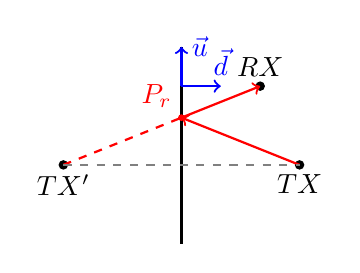
\begin{tikzpicture}[scale=0.5]
        \draw[thick] (1, -1) -- (1, 4);
        \filldraw[black] (4, 1) circle (3pt) node[anchor=north] {$TX$};
        \filldraw[black] (3, 3) circle (3pt) node[anchor=south] {$RX$};
        \filldraw[black] (-2, 1) circle (3pt) node[anchor=north] {$TX'$};
        \draw[red, thick, dashed] (-2, 1) -- (1, 2.2) node[midway, above] {};
        \draw[red, thick, ->] (1, 2.2) -- (3, 3) node[midway, above] {};
        \draw[red, thick, ->] (4, 1) -- (1, 2.2) node[midway, above] {};
        \filldraw[red] (1, 2.2) circle (2pt) node[anchor=south east] {$P_r$};
        \draw[->, blue, thick] (1, 3) -- (1, 4) node[anchor=west] {$\vec{u}$};
        \draw[->, blue, thick] (1, 3) -- (2, 3) node[anchor=south] {$\vec{d}$};
        
        \draw[gray, thick, dashed] (-2, 1) -- (4, 1);
        
    \end{tikzpicture}
    \caption{Antenne image $TX'$ de l'émettrice $TX$}
    \label{fig:antenne_image}
\end{figure}
\subsection{Cas à deux réflexions}
Pour le cas à deux réflexions, il suffit de prendre d'abord en compte l'image du premier mur sur lequel on se reflète ($I_1$ sur le schéma), et puis à partir de ce point image, on détermine son propre point image par rapport au second mur sur lequel on se reflète ($I_2$). 

On considère alors que le point de réflexion sur le second mur ($Pr_2$) est l'intersection entre ledit mur et le récepteur, et pour le premier point de réflexion ($Pr_{1}$), il s'agit de l'intersection entre la première image et $Pr_{2}$. 
Ceci est illustré sur la figure  \ref{fig:reflexion_double}. Il est pertinent de noter que la distance totale du rayon (composé des trois traits verts) est égale à la distance entre le récepteur ($RX$) et le dernier point image ($I_2$).

\begin{figure}[H]
    \centering
    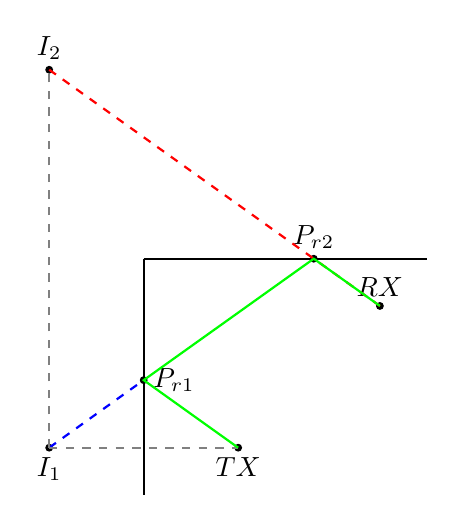
\begin{tikzpicture}[scale=.6]
    \draw[thick] (0, 0) -- (0, 5);
    \draw[thick] (0, 5) -- (6, 5);

    \filldraw (2, 1) circle (2pt) node[anchor=north] {$TX$};
    \filldraw (5, 4) circle (2pt) node[anchor=south] {$RX$};

    \filldraw (-2, 1) circle (2pt) node[anchor=north] {$I_1$};
    \filldraw (-2, 9) circle (2pt) node[anchor=south] {$I_2$};

    \filldraw (0, 2.43) circle (2pt) node[anchor=west] {$P_{r1}$};
    \filldraw (3.6, 5) circle (2pt) node[anchor=south] {$P_{r2}$};
    \draw[red, thick, dashed] (-2, 9) -- (5, 4);
    \draw[blue, thick, dashed] (-2, 1) -- (0, 2.43);
    \draw[gray, thick, dashed] (-2, 1) -- (-2, 9);
    \draw[gray, thick, dashed] (-2, 1) -- (2, 1);
    
    \draw[green, thick] (2, 1) -- (0, 2.43) -- (3.6, 5) -- (5, 4);
    \end{tikzpicture}
    \caption{Méthode des images pour deux réflexions entre $TX$ et $RX$}
    \label{fig:reflexion_double}
\end{figure}